%====================================================================================================
% ?????
%====================================================================================================
% TCC
%----------------------------------------------------------------------------------------------------
% Autor				: Jasane Schio
% Orientador		: Gedson Faria
% Co-Orientador		: Angelo Darcy
% Instituição 		: UFMS - Universidade Federal do Mato Grosso do Sul
% Departamento		: CPCX - Sistema de Informação
%----------------------------------------------------------------------------------------------------
% Data de criação	: 01 de Outubro de 2015
%====================================================================================================
% NO FUTURO
\chapter{Resultados} 


	Para serem feitos os testes foram despostos no campo tiras coloridas entre 17 e 40 centimetros de largura e  5,5 e 10,5 centimetros de altura. Cada cor possue três tiras, e cada uma das tiras foi colocada em uma parte do campo que foi dividio em três.


Para a execução dos tipos de testes, o campo foi dividido verticalmente em cinco partes, de vinte e nove centimetros cada, e horizontalmente em três parte de quarenta e um centimetro cada, somando um total de quinze areas de calibração, nomeadas alfabeticamente de A à O, como mostrado na Figura \ref{campodivisao}.

\begin{figure}[!: h]
		\centering
		\includegraphics[width=0.3\textwidth]{campodivisao.pdf}
		\caption{Divisao do campo em quinze partes nomeadas alfabeticamente.}
		\label{campodivisao}
	\end{figure}
	
Em cada areas de calbração estão dispostas cinco cores: Vermelho  e Verde na primeira linha, Amarelo, Azul e Laranja na segunda. As cores estão distantes verticalmente \textit{7.5cm}, na primeria linha a distancia entre as cores é  de \textit{11 cm} e na segunda linha de \textit{7.2 cm}. Um  melhor detalhamento da disposiçao das cores é  mostrado na Figura \ref{disposicaoparte}. No total estavam disposto no campo quinze pontos de cada cor.


MUDAR ESSA FIGRURA
\begin{figure}[H]
		\centering
		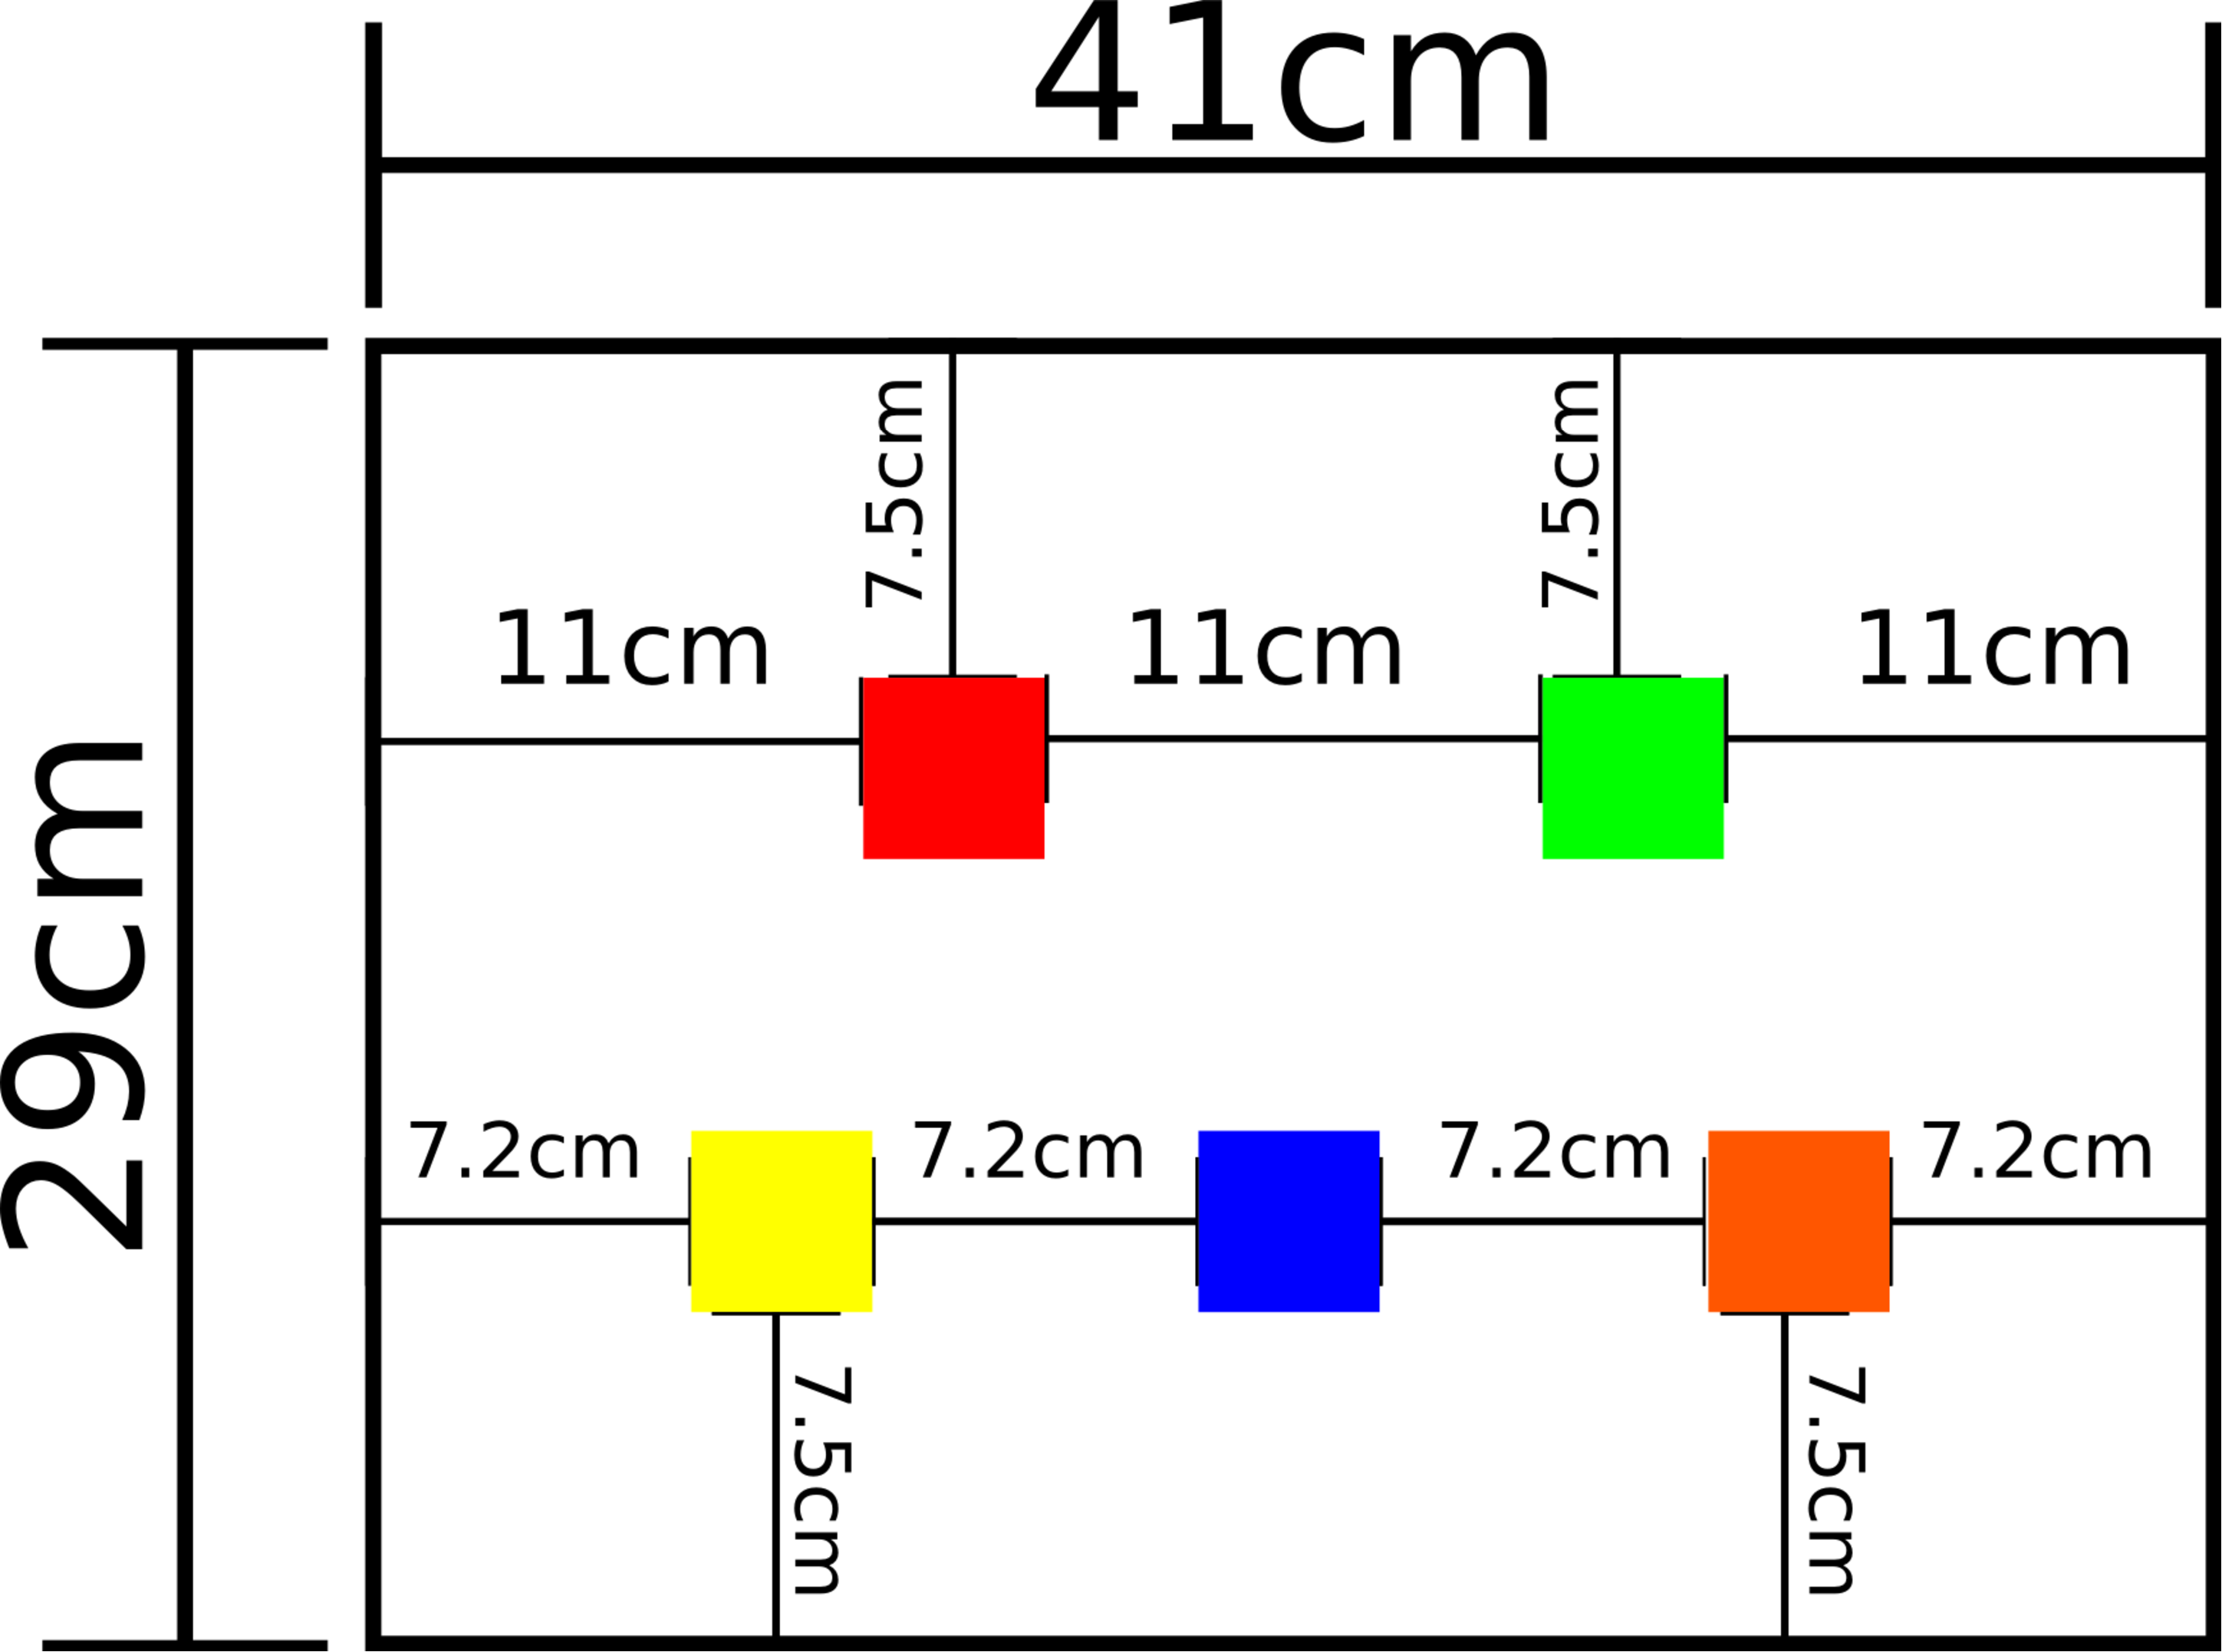
\includegraphics[width=0.3\textwidth]{disposicaoparte.pdf}
		\caption{Disposição dos objetos coloridos dentro de cada uma das partes}
		\label{disposicaoparte}
	\end{figure}

	
A realização da aquisição de minimos ocorreu dia 19 de Agosto de 2016, entre 17:36 e 17:39.

Seleção de Campo:
\begin{figure}[H]
		\centering
		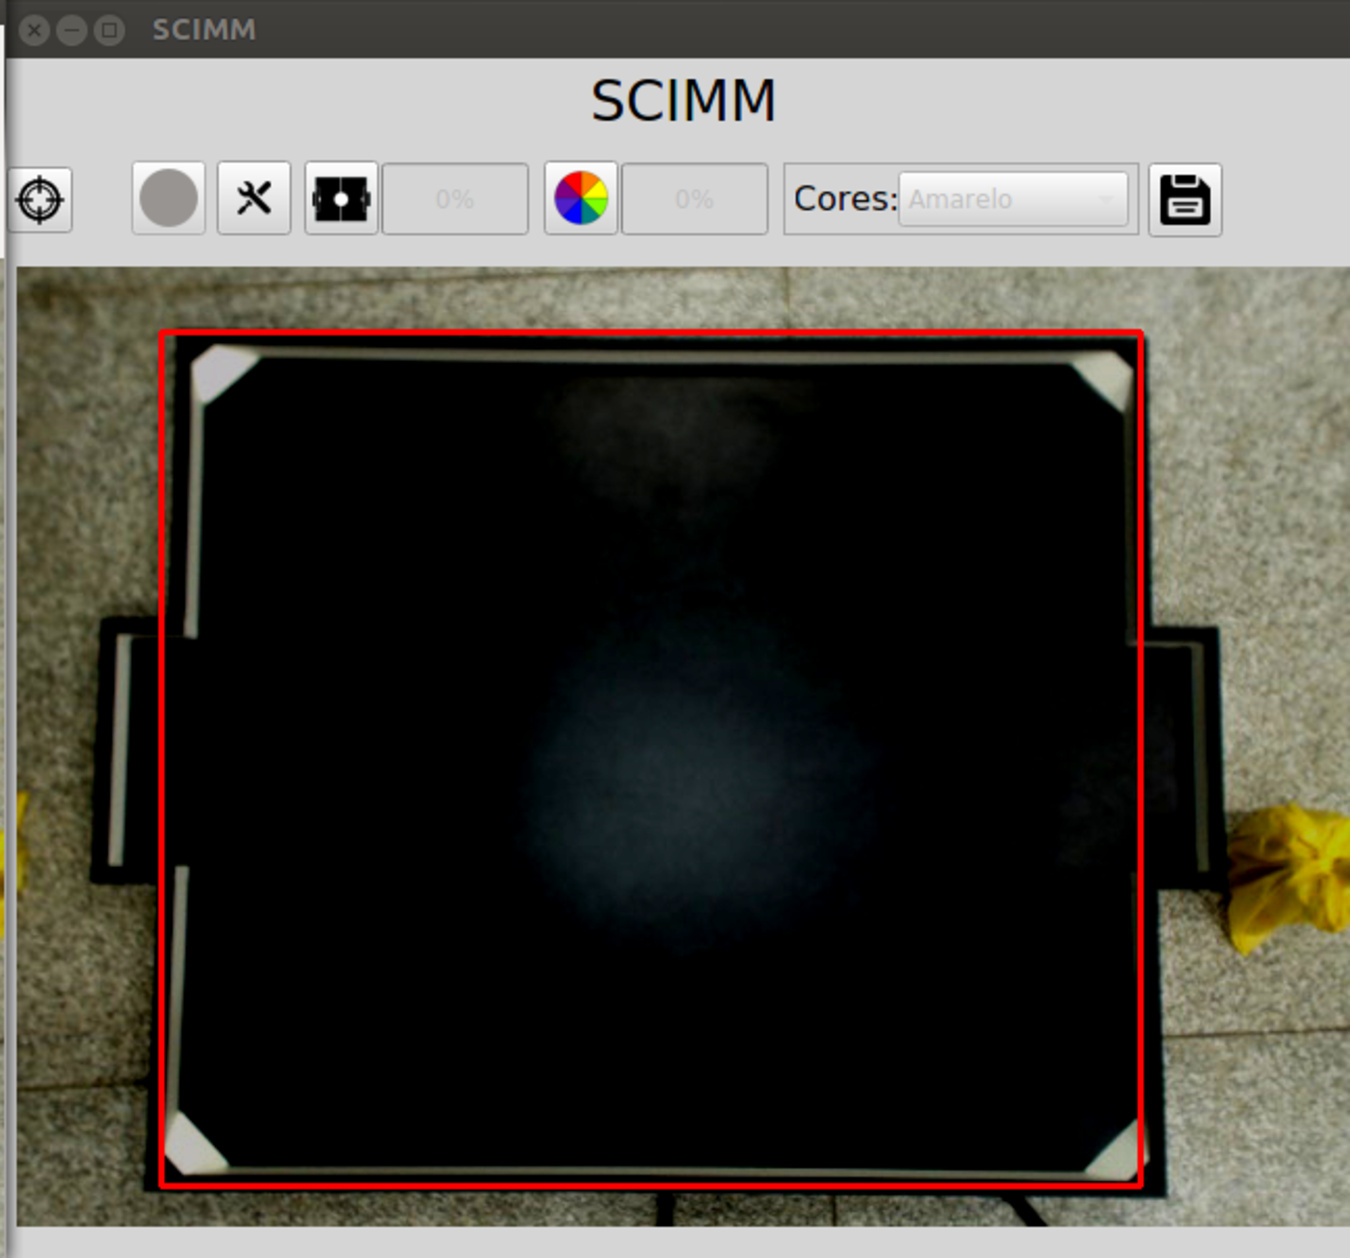
\includegraphics[width=0.7\textwidth]{fundoteste.pdf}
		\caption{Imagem do fundo com a seleção de campo}
		\label{disposicaoparte}
	\end{figure}
	
Imagem dos objetos dispostos:
	\begin{figure}[H]
		\centering
		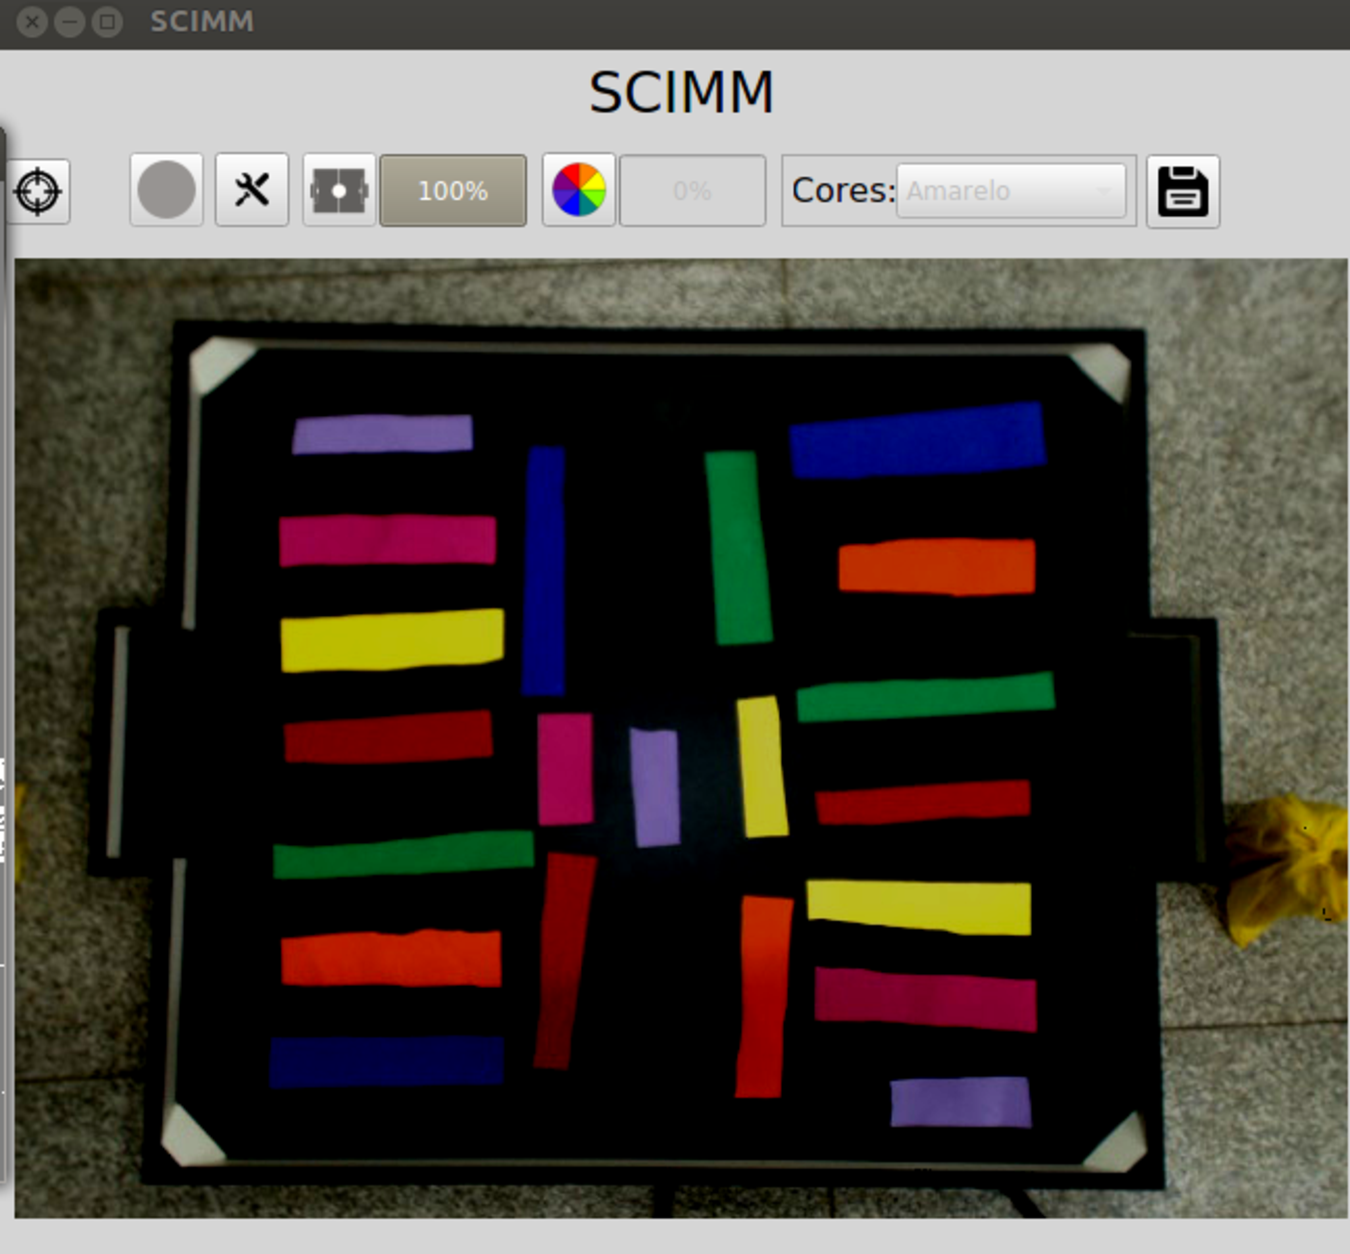
\includegraphics[width=0.7\textwidth]{objetosdispostos.pdf}
		\caption{Objetos dispostos no campo para calibração}
		\label{disposicaoparte}
	\end{figure}
	
Mascara gerada a partir da subtração de fundo:
	\begin{figure}[H]
		\centering
		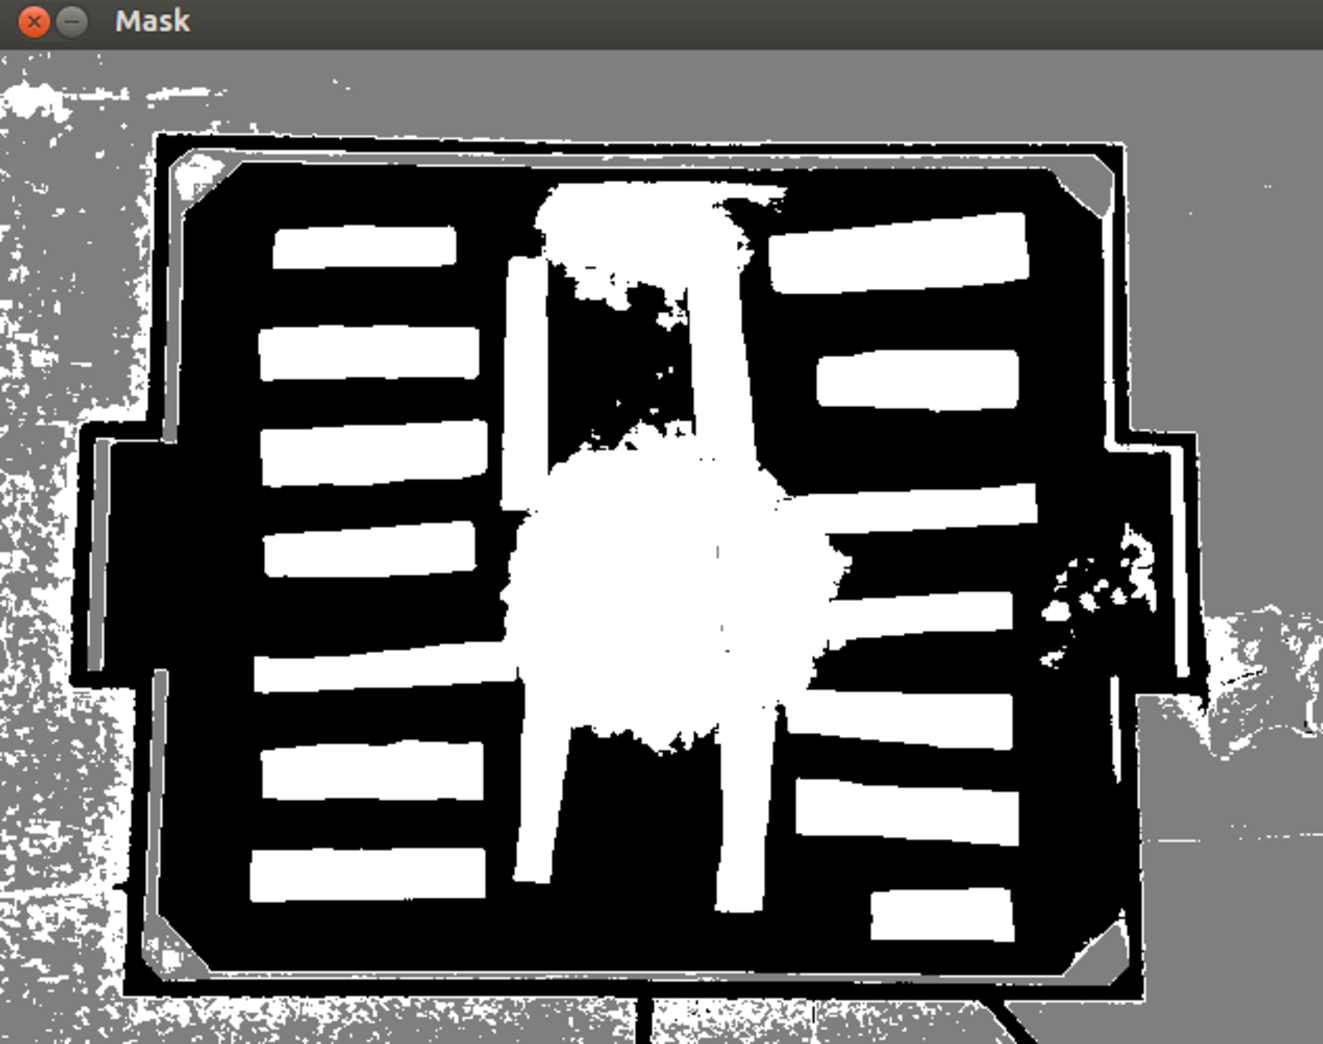
\includegraphics[width=0.7\textwidth]{mascaragerada.pdf}
		\caption{Objetos dispostos no campo para calibração}
		\label{disposicaoparte}
	\end{figure}
	
Arquivo \textit{cores.arff} gerado:
\begin{center}
21.100.100 \newline
30.255.255\newline
92.100.100\newline
120.255.255\newline
62.100.100\newline
90.255.255\newline
169.100.100\newline
179.255.255\newline
0.100.100\newline
20.255.255\newline
161.100.100\newline
168.255.255\newline
126.0.0\newline
160.255.255\newline

\end{center}

	